\documentclass[../EngineeringJournal_CDavis.tex]{subfiles}

\begin{document}

%%%%%%%%%%%%%%%%%%%%%%%%%%%%%%%%%%%%%%%%%%%%%%%%%%%%%
%%%%%%%%%%%%%%%%%%%%%%%%%%%%%%%%%%%%%%%%%%%%%%%%%%%%%

\chapter[Configuring Basic Router]{Configuring Basic \linebreak[1] Router Settings \hspace*{\fill}{Jan 23, 2020}}
\noindent\textbf{{Packet Tracer Lab 1} \hspace*{\fill}{\textbf{CIT 167}}}\linebreak[1]
{{Spring 2020} \hspace*{\fill}{Chaz Davis}}                             %===================================

\hspace{0.2cm}
\begin{tcolorbox}[width=6.3in]
\scriptsize 
- Important Commands for the Lab
  \begin{itemize}
    \item{no ip domain lookup} suppresses all DNS-lookups from the router to the configured DNS seves
      \subitem{allows for sloppy typing} keeps from doing a lookup everytime
      \subitem{better practice} configure ip name-server
      \subitem{then disable automatic telnetting to ``hostnames''"}
      \subitem{transport prefferred none} and set that for con, aux, and vty
    \item{exec-timeout 5 0}
      \subitem{configure the inactive session timeout on console port}
      \subitem{parameter passed in is minutes}
      \subitem{if two nubers passed the second is seconds}
    \item{logging synchronous}
      \subitem{for when long commands are interrupted by console message}
      \subitem{tells the router to hold messages until it detects no input from the keyboard}
    \item{service password-encryption} 
      \subitem{normally all passwords, except enable secret, are stored in clear-text}
      \subitem{stores all passwords in an encrypted form}
      \subitem{stores them using an MD5 hashing algorithm}
    \item{?} allows you to look up help from commandline 
      \subitem{similar to --help on linux}
      \subitem{if no help available, returns <CR>}
  \end{itemize}
- Important Concepts
  \begin{itemize}
    \item{Understand the process of setting up new schemes}
    \item{Logging in over ssh and telnet from the commandline}
    \item{Finding info through the long lines of output}
  \end{itemize}
\end{tcolorbox}
\hspace{0.2cm}
\normalsize  

\newpage

%===================================
\mysection{\textbf{Part 1:Set Up the Topology}}

\mysubsection{1}{Cable the Network}
I started off by placing the the router(1941), the switch(2960), and 2 windows 7 pcs on the the canvas.


\begin{figure}[!hbt]
  \centering
  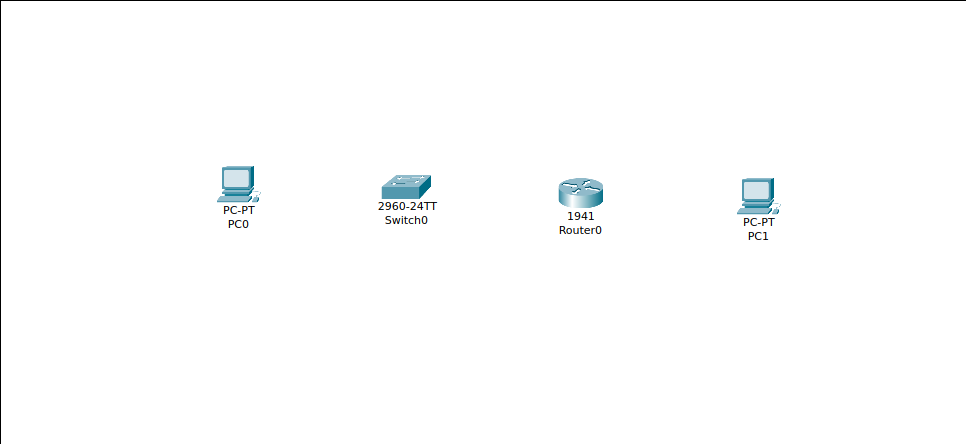
\includegraphics[width=.45\linewidth]{Figures/2020-01-28-090220_966x444_scrot.png}
  \caption{View of the Network Topology}
  \label{Topo1}
\end{figure}

\noindent\mysubsection{2}{Wiring up the routers}
\\Next I used straight copper wiring to connect the router the switch and the two pcs
and renamed the accordingly. See Fig~\ref{netconfig1}.

\begin{figure}[!hbt]
  \begin{minipage}[c]{0.4\linewidth}
    \centering
    \begin{tabular}{|l|l|l|}
        Device & connected on & connected to \\
        \hline
        PC-A & FA0 & S1 Fa0/6 \\
        S1 & Fa0/6 & PC-A Fa0/6 \\
        R1 & gig 0/1 & S1 Fa0/5 \\
        PC-B & FA0 & R1 gig0/0 
    \end{tabular}
    \subcaption{IP table}\label{netconfig1table1}
  \end{minipage}\hfill
  %
  \begin{minipage}[c]{0.4\linewidth}
    \centering
    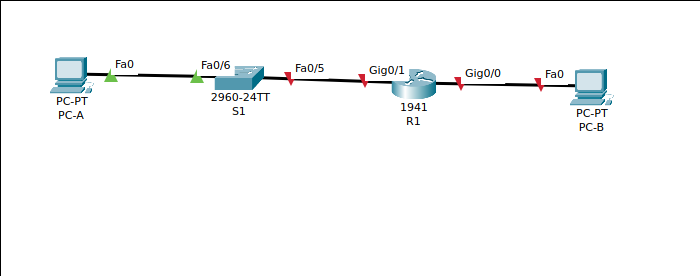
\includegraphics[scale=0.3]{Figures/2020-01-28-092436_700x276_scrot.png}
    \subcaption{Showing the Network}\label{netconfig1scrot1}
  \end{minipage}
  \caption{Configuring the Network}\label{netconfig1}
\end{figure}

%===================================
\mysection{\textbf{Part 2: Configure Devices and Verify connectivity}}
I started off by configuring the ipaddress, subnet mask, and default gateways on PC-A and PC-B
\hfill\break

\noindent\mysubsection{1}{Configuring the PCs}
I started off by configuring the IPs for the PC's. See Fig~\ref{config1}.

\begin{figure}[!hbt]
  \begin{minipage}[c]{0.4\linewidth}
    \centering
      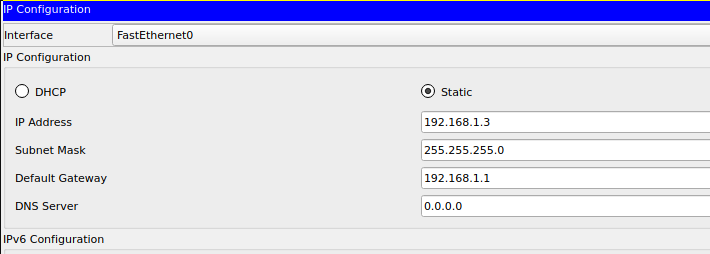
\includegraphics[scale=0.24]{Figures/2020-01-28-093105_710x254_scrot.png}
      \subcaption{IP Config PC-A}\label{config1PC-a}
  \end{minipage}\hfill
  %
  \begin{minipage}[c]{0.4\linewidth}
    \centering
    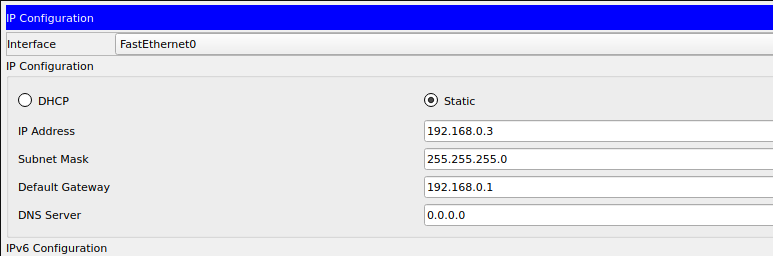
\includegraphics[scale=0.24]{Figures/2020-01-28-093427_773x256_scrot.png}
    \subcaption{IP Config PC-B}\label{config1PCb}
  \end{minipage}
  \caption{Configuring the IPs}\label{config1}
\end{figure}

\clearpage

\noindent\mysubsection{2}{Configuring the router}
\\Next I logged into the router went to the commandline, and escalated to priveledged exec mode.

\hfill\break

\subsubsection{1}{Name and passwords}

\begin{mdframed}
\scriptsize
\begin{verbatim}
Router>ena
Router#conf t
Enter configuration commands, one per line.  End with CNTL/Z.
Router(config)#hostname R1
R1(config)#no ip domain lookup
R1(config)#no ip domain-lookup
R1(config)#security passwords min-length 10
R1(config)#enable secret cisco12345
R1(config)#line con 0
R1(config-line)#password coscoconpass
R1(config-line)#exec-timeout 5 0
R1(config-line)#login
R1(config-line)#logging synchronous
R1(config-line)#exit
R1(config)#line vty 0 4
R1(config-line)#password ciscovtypass
R1(config-line)#exec-timeout 5 0
R1(config-line)#login
R1(config-line)#logging synchronous
R1(config-line)# exit
R1(config)#service password-encryption
R1(config)#banner motd #Unauthorized access prohibited!#
\end{verbatim}
\normalsize
\end{mdframed}

\subsubsection{2}{Connections}
\begin{multicols}{2}
\begin{mdframed}
\scriptsize
\begin{verbatim}
R1(config)#int g0/0
R1(config-if)#description Connection to PC-B
R1(config-if)#ip address 192.168.0.1 255.255.255.0
R1(config-if)#no shut

R1(config-if)#
%LINK-5-CHANGED: Interface GigabitEthernet0/0,
changed state to up

%LINEPROTO-5-UPDOWN: Line protocol on Interface 
GigabitEthernet0/0, changed state to up

R1(config-if)#exit
R1(config)#exit
R1#
%SYS-5-CONFIG_I: Configured from console by console

R1#clock set 10:00:00 28 Jan 2020
R1#copy running-config startup-config
Destination filename [startup-config]? 
Building configuration...
[OK]
R1#
\end{verbatim}
\normalsize
\end{mdframed}

I then did the same for PC-A
\begin{mdframed}
\scriptsize
\begin{verbatim}
R1(config)#int g 0/1
R1(config-if)#description Connection to S1
R1(config-if)#ip address 192.168..1.1 255.255.255.0
                         ^
% Invalid input detected at '^' marker.
	
R1(config-if)#ip address 192.168.
                         ^
% Invalid input detected at '^' marker.
	
R1(config-if)#ip address 192.168.1.1 255.255.255.0
R1(config-if)#no shut

R1(config-if)#
%LINK-5-CHANGED: Interface GigabitEthernet0/1,
changed state to up

%LINEPROTO-5-UPDOWN: Line protocol on Interface 
GigabitEthernet0/1, changed state to up

R1(config-if)#
\end{verbatim}
\normalsize
\end{mdframed}
\end{multicols}

\clearpage
%===================================

\subsubsection{3}{Verifying network connectivity}

\begin{figure}[!hbt]\centering
  \subfloat[R1 Enable]{\label{Verify1R1}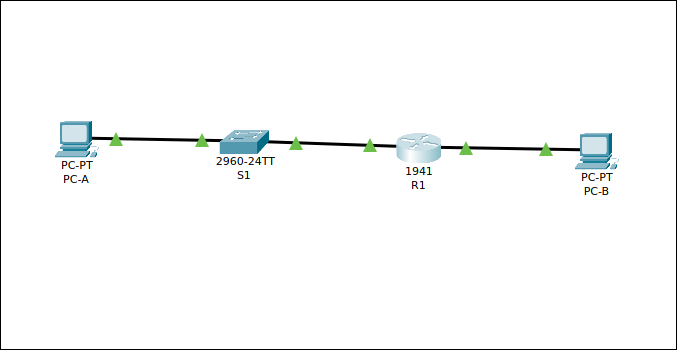
\includegraphics[width=.45\linewidth]{Figures/2020-01-28-100133_679x351_scrot.png}}\par
  \subfloat[Pingin PC-B from PC-A]{\label{Verify1AtoB}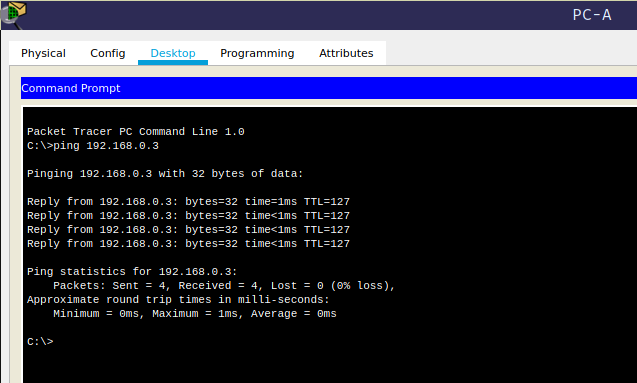
\includegraphics[width=.36\linewidth]{Figures/2020-01-28-100457_637x383_scrot.png}}\hfill
  \subfloat[Telnet PC-A to R1]{\label{Verify1AtoR}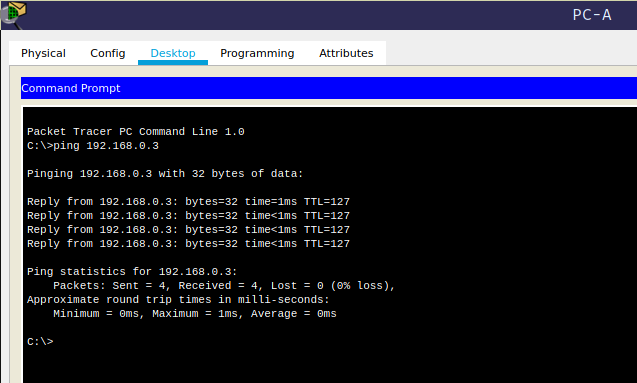
\includegraphics[width=.36\linewidth]{Figures/2020-01-28-100457_637x383_scrot.png}}
\caption{Verifying the Network Connectivity}
\label{Verify1}
\end{figure}


%===================================
\mysection{\textbf{Part 3: Display Router Information}}
\mysubsection{1}{important hardware and software info}
\\While logged in with telnet I ran the following commands
\begin{mdframed}
\scriptsize
\begin{verbatim}
R1>show version
Cisco IOS Software, C1900 Software (C1900-UNIVERSALK9-M), 
Version 15.1(4)M4, RELEASE SOFTWARE (fc2)
Technical Support: http://www.cisco.com/techsupport
Copyright (c) 1986-2007 by Cisco Systems, Inc.
Compiled Wed 23-Feb-11 14:19 by pt_team

ROM: System Bootstrap, Version 15.1(4)M4, RELEASE SOFTWARE (fc1)
cisco1941 uptime is 1 hours, 19 minutes, 11 seconds
System returned to ROM by power-on
System image file is "flash0:c1900-universalk9-mz.SPA.151-1.M4.bin"
Last reload type: Normal Reload

This product contains cryptographic features 
and is subject to United States and local country 
laws governing import, export, transfer and
use. Delivery of Cisco cryptographic products does not imply
third-party authority to import, export, 
distribute or use encryption. Importers, exporters, 
distributors and users are responsible for
compliance with U.S. and local country laws. 
By using this product you agree to comply with 
applicable laws and regulations. If you are unable to 
comply with U.S. and local laws, 
return this product immediately.

A summary of U.S. laws governing Cisco 
cryptographic products may be found at:
http://www.cisco.com/wwl/export/crypto/tool/stqrg.html

\end{verbatim}
\normalsize
\end{mdframed}

We can see that  the IOS image on the router is Cisco IOS Software,

\begin{mdframed}
\scriptsize
\begin{verbatim}
C1900 Software (C1900-UNIVERSALK9-M), Version 15.1(4)M4, RELEASE SOFTWARE (fc2)
\end{verbatim}
\normalsize
\end{mdframed}

We can also see that the NVRAM by using show flash:

\begin{mdframed}
\scriptsize
\begin{verbatim}
R1#show flash 

System flash directory:
File  Length   Name/status
  3   33591768 c1900-universalk9-mz.SPA.151-4.M4.bin
  2   28282    sigdef-category.xml
  1   227537   sigdef-default.xml
[33847587 bytes used, 221896413 available, 255744000 total]
249856K bytes of processor board System flash (Read/Write)
\end{verbatim}
\normalsize
\end{mdframed}

\mysubsection{2}{Display Startup Info}
\begin{mdframed}
\scriptsize
\begin{verbatim}
R1#show startup-config
Using 959 bytes
!
version 15.1
no service timestamps log datetime msec
no service timestamps debug datetime msec
service password-encryption
security passwords min-length 10
!
hostname R1
!
enable secret 5 $1$mERr$WvpW0n5HghRrqnrwXCUUl.
!
ip cef
no ipv6 cef
!
license udi pid CISCO1941/K9 sn FTX1524C630-
no ip domain-lookup
spanning-tree mode pvst
!
interface GigabitEthernet0/0
 description Connection to PC-B
 ip address 192.168.0.1 255.255.255.0
 duplex auto
 speed auto
!
interface GigabitEthernet0/1
 no ip address
 duplex auto
 speed auto
 shutdown
!
interface Vlan1
 no ip address
 shutdown
!
ip classless
ip flow-export version 9
banner motd ^CUnauthorized access prohibited!^C
!
line con 0
 exec-timeout 5 0
 password 7 0822435D0A1606181C1B0D1739
 logging synchronous
 login
!
line aux 0
!
line vty 0 4
 exec-timeout 5 0
 password 7 0822455D0A1613030B1B0D1739
 logging synchronous
 login
!
end
\end{verbatim}
\normalsize
\end{mdframed}

From this we can see that the passwords are encrypted

I used show startup-config | begin vty
\\It did not like that command wouldnt show any info

\mysubsection{3}{Display the routing table on the router}
\\ i ran show ip route
\begin{mdframed}
\scriptsize
\begin{verbatim}
R1#show ip route
Codes: 
L - local, C - connected, S - static, R - RIP, M - mobile, B - BGP
D - EIGRP, EX - EIGRP external, O - OSPF, IA - OSPF inter area
N1 - OSPF NSSA external type 1, N2 - OSPF NSSA external type 2
E1 - OSPF external type 1, E2 - OSPF external type 2, E - EGP
i - IS-IS, L1 - IS-IS level-1, L2 - IS-IS level-2,
ia - IS-IS inter area
* - candidate default, U - per-user static route, o - ODR
P - periodic downloaded static route

Gateway of last resort is not set

  192.168.0.0/24 is variably subnetted, 2 subnets, 2 masks
C 192.168.0.0/24 is directly connected, GigabitEthernet0/0
L 192.168.0.1/32 is directly connected, GigabitEthernet0/0
  192.168.1.0/24 is variably subnetted, 2 subnets, 2 masks
C 192.168.1.0/24 is directly connected, GigabitEthernet0/1
L 192.168.1.1/32 is directly connected, GigabitEthernet0/1

R1#
\end{verbatim}
\normalsize
\end{mdframed}

There are two entries with a C encoding

\mysubsection{4}{Display a summary list}
Display a summary list of the interfaces on the router
\\I ran the show ip interface brief command:

\begin{mdframed}
\scriptsize
\begin{verbatim}
show ip interface brief
Interface           IP-Address  OK? Method Status           Protocol 
GigabitEthernet0/0  192.168.0.1 YES manual up                    up 
GigabitEthernet0/1  192.168.1.1 YES manual up                    up 
Vlan1               unassigned  YES unset  administratively down down
\end{verbatim}
\normalsize
\end{mdframed}

when we gave the command `no shut` that changed the gig ethernet ports from down to up.

\end{document}
